\section{Mathematical Modeling}

\subsection{Equations of Motion}
The equations of motion for the pitch, travel- and elevation angle were derived on the basis of Newton's second law for rotation:
%
\begin{equation}
    \sum \vec{\tau}_{z} = \sum \vec{r}_i\times\vec{F}_i = \sum(\vec{m_i}\vec{r_i^2})\vec{\alpha}_z= J\alpha_z \label{EOR}
\end{equation}
%

%
Where $\vec{\tau}$ is the torque about the given axis (z), $\alpha$ is the angular acceleration and $J$ is the moment of inertia around the given point, given a rigid body and that the cross-product is defined \cite{uniphysics}.
In our assignement we used the illustrations shown in \cref{fig:illustrasjon} as a basis for our mathematical models.\\ Also given were the relations between the forces and voltages and equations for the moments of inertia for each joint:
%
\begin{subequations}
    \begin{align}
    F_f &= K_fV_f   \nonumber              \\
    F_b &= K_fV_b   \nonumber               \\ \nonumber \\
    J_p &= 2m_pl_p^2                           \label{eq:MOI1} \\
    J_e &= m_cl_c^2 + 2m_pl_h^2                \label{eq_MOI2}\\
    J_\lambda &= m_cl_c^2 + 2m_p(l_h^2+l_p^2)  \label{eq:MOI3}  %\tag{2c}
    \end{align}
\end{subequations}
%
\begin{figure}[b]
    \centering
    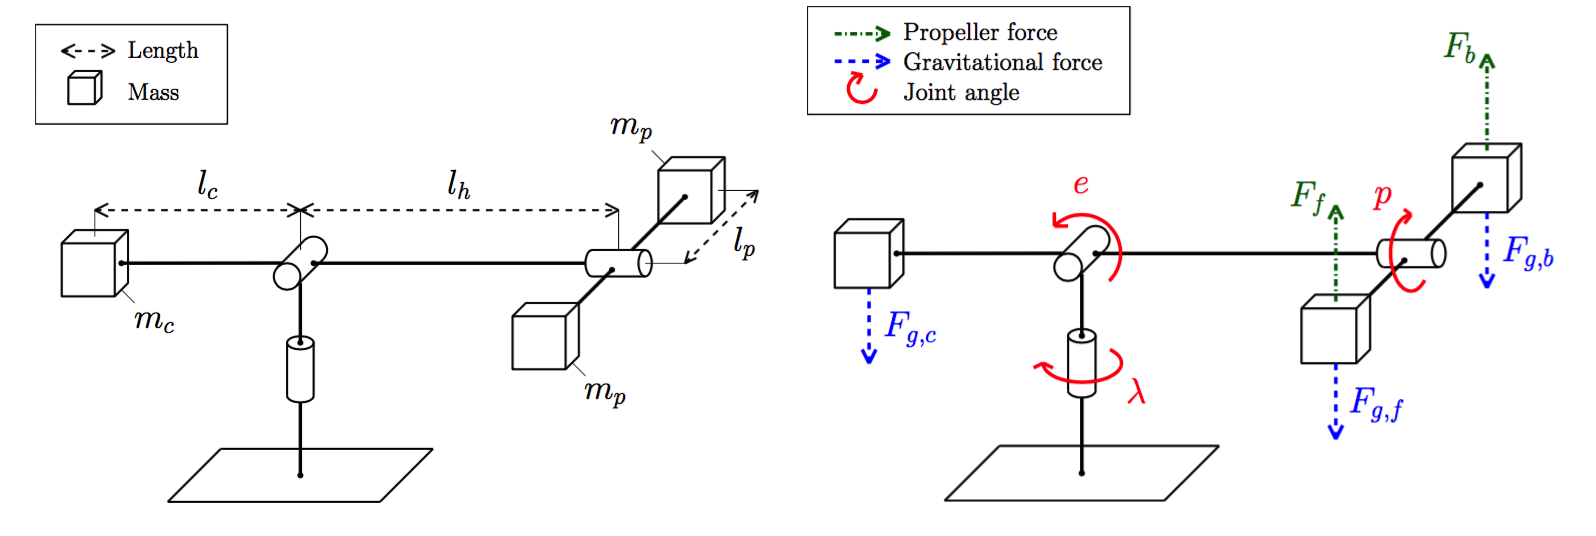
\includegraphics[width=1.0\textwidth]{helikopter.png}
    \caption{Illustration and free body diagram of our helicopter model. Image credit: \cite{labtext}}
    \label{fig:illustrasjon}
\end{figure}
Here $p$ is the pitch angle, $e$ is the elevation angle, $\lambda$ is the travel angle and $J_x$ is the respective moment of intertia.

%%%%%%%%%%%%%%%%%%%%%%%%%%%%%%%%%%%%%%%%%%%%%%%%%%%%%%%%%%%%%%%%%%%%%%

\subsubsection*{Pitch (p) :}
\begin{align*}
    \sum\vec{\tau_p} &= l_p(F_f-F_b) + l_p\cos(p)(F_{g,p}-F_{g,f})\\
     &= l_pK_f(V_f-V_b) 
\end{align*}
Then using Newton's 2nd. law of rotation (eq.\ref{EOR}):
\begin{equation}
    J_p\ddot{p} = l_pK_fV_d = L_1V_d \tag{3a}\label{3a}
\end{equation}

%%%%%%%%%%%%%%%%%%%%%%%%%%%%%%%%%%%%%%%%%%%%%%%%%%%%%%%%%%%%%%%%%%%%%%

\subsubsection*{Elevation (e) :}
\begin{align*}
    \sum\vec{\tau} &= l_h(F_f+F_b) + [-l_h(F_{g,f}+F_{g,b})]\cos(e) + l_cF_{g,c}\cos(e)\\
    &= l_hK_fV_s\cos(p) + g\cos(e)(l_cm_c - 2l_hm_p)
\end{align*}
Then from (eq.\ref{EOR}):
\begin{equation}
    J_e\ddot{e} = L_3V_s\cos(p) + L_2\cos(e) \tag{3b} \label{3b}
\end{equation}

%%%%%%%%%%%%%%%%%%%%%%%%%%%%%%%%%%%%%%%%%%%%%%%%%%%%%%%%%%%%%%%%%%%%%%

\subsubsection*{Travel ($\lambda$) :}
\begin{align*}
    \sum\vec{\tau} &= -l_h(F_f+F_b)\sin(p)\cos(e)\\
    &= -l_hK_fV_s\sin(p)\cos(e)
\end{align*}
Which again leaves us with
\begin{equation}
    J_\lambda\ddot{\lambda} = L_4V_s\sin(p)\cos(e) \tag{3c}\label{3c}
\end{equation}


%%%%%%%%%%%%%%%%%%%%%%%%%%%%%%%%%%%%%%%%%%%%%%%%%%%%%%%%%%%%%%%%%%%%%%
\newpage %??
\subsection{Linearization}
We want to linearize the system around the given point of equilibrium $(p, e, \lambda)^T$ = $[p^*, e^*, \lambda^*]^T = (0, 0, 0)^T \quad \forall t \quad\Rightarrow\quad [\ddot{p},\ddot{e},\ddot{\lambda}]^T = (0,0,0)^T$. Inserting  \cref{3a}-(\ref{3c}) into $(V_s,V_c)^T = (V_s^{*},V_d^{*})^T$ gives us
%
\begin{align*}
    V_{s,e}^* = -\frac{L_2}{L_3}&\frac{\cos(e)}{\cos(p)} = -\frac{L_2}{L_3}\\
    V_{s,\lambda}^* &= 0\\
    0 = l_pK_fV_d^* \quad &\Rightarrow\quad V_d^* = 0\\
    \Rightarrow\begin{bmatrix}V_s^* \\ V_d^*\end{bmatrix} &= \begin{bmatrix}-\frac{L_2}{L_3}\\0\end{bmatrix} 
\end{align*}
%
We now introduce the coordinate transformation
\setcounter{equation}{3}
%
\begin{align*}
    \begin{bmatrix}\widetilde{p}\\\widetilde{e}\\\widetilde{\lambda} \end{bmatrix}
    = \begin{bmatrix}p\\e\\\lambda\end{bmatrix}
    - \begin{bmatrix}p^*\\e^*\\\lambda^*\end{bmatrix}
    \quad\text{and}\quad
    \begin{bmatrix}\tilde{V_s}\\\tilde{V_d} \end{bmatrix}
    = \begin{bmatrix}V_s\\V_d\end{bmatrix}
    - \begin{bmatrix}V_s^*\\V_d^*\end{bmatrix}  %\tag{4}
\end{align*}
%
The equations \ref{3a} - \ref{3c} then transform into
%
\setcounter{equation}{3}
\begin{align}
    \begin{bmatrix}\widetilde{p}\\\widetilde{e}\\\widetilde{\lambda} \end{bmatrix}
    = \begin{bmatrix}\frac{L_1}{J_p}(\tilde{V_d}+V_d^*) - p^*  \\ 
    \frac{L_2}{J_e}\cos(\widetilde e + e^*)+\frac{L_3}{J_e}(\tilde{V_s}+V_s^*)\cos(\widetilde{p}+p^*) - e^*  \\  
    \frac{L_4}{J_\lambda}(\tilde{V_s}+V_s^*)\cos(\widetilde{e}+e^*)\sin(\widetilde{p}+p^*) - \lambda^*  \end{bmatrix} %\tag{5}
\end{align}
%
Defining the states and input as $\vec{x} = [\widetilde{p},\widetilde{e},\widetilde{\lambda}]^T$ and $\vec{u} = [\tilde{V_s},\tilde{V_d}]^T$ giving $\vec{h} = \vec{h}(\vec{x},\vec{u}) = [\ddot{\widetilde{p}},\ddot{\widetilde{e}},\ddot{\widetilde{\lambda}}]^T$ around the equilibrium point $(x_0,u_0)$. The transformed system can them be written in a state-space form \cite{chen2014linear}:
%
\begin{align*}
    \vec{\widetilde{x}} = \vec{A}\vec{x} + \vec{B}\vec{u}
\end{align*}
%
where 
%
\begin{align*}
    \vec{A} = \frac{\partial\vec{h}}{\partial\vec{x}}\bigg|_{(x_0,u_0)}
    \quad\text{and}\quad
    \vec{B} = \frac{\partial\vec{h}}{\partial\vec{u}}\bigg|_{(x_0,u_0)}
\end{align*} 
%
This results in the state-space model
%
\begin{align}
    \vec{\ddot{x}} = 
    \begin{bmatrix}0&0&0\\0&0&0\\\frac{L_4}{J_\lambda}&0&0
    \end{bmatrix}
    \vec{x} + 
    \begin{bmatrix}0&\frac{L_1}{J_p}\\\frac{L_3}{J_3}&0\\0&0
    \end{bmatrix}
    \vec{u} %\tag{6}\label{eq.6}
\end{align}
%
Which corresponds to
\begin{subequations}
\begin{align}
    \ddot{\widetilde{p}} &= \frac{L_1}{J_p}\tilde{V_d} = K_1\tilde{V_d}   \\%\tag{7a}\\
    \ddot{\widetilde{e}} &= \frac{L_3}{J_e}\tilde{V_s} = K_2\tilde{V_s}   \\%\tag{7b}\\
    \ddot{\widetilde{\lambda}} &= \frac{L_4}{J_\lambda}\tilde{V_s^*}\widetilde{p} = K_3\widetilde{p} \label{eq:6c}
\end{align}
\end{subequations}

%%%%%%%%%%%%%%%%%%%%%%%%%%%%%%%%%%%%%%%%%%%%%%%%%%%%%%%%%%%%%%%%%%%%%%
\subsection{Physical Behaviour Around Equilibrium}

Since linearization of non-linear systems only provide an approximation of the model in question, it is valid mostly around the defined operating point (equilibrium), but breaks if one deviates too far. This holds for feedforward and other types of linearized controllers. We had a hard time controlling the helicopter using just feedforward control, possibly slightly better performance around the equilibrium, but difficult to notice. The helicopter was also seemingly eager to oscillate given small pitch adjustments. 

%%%%%%%%%%%%%%%%%%%%%%%%%%%%%%%%%%%%%%%%%%%%%%%%%%%%%%%%%%%%%%%%%%%%%%

\subsection{Determining the Motor Force Constant}
The motor force constant $K_f$ was determined by firstly measuring the the voltage $V_s = V_s^*$ which kept the helicopter at equilibrium $(e = e^* = 0)$. $V_s$ was measured to be $7.2 $ V. The values for $e$ and $V_s$ was then inserted into (\ref{3b}) resulting in 
%
\begin{align*}
    K_f = -g\dfrac{l_cm_c-2l_hm_p}{V_sl_h} = \underline{0.1387}.
\end{align*}
%
This value is used in the following problems.

